\documentclass{article}


\usepackage{arxiv}

\usepackage[utf8]{inputenc} % allow utf-8 input
\usepackage[T1]{fontenc}    % use 8-bit T1 fonts
\usepackage{hyperref}       % hyperlinks
\usepackage{xurl}            % simple URL typesetting
\usepackage{booktabs}       % professional-quality tables
\usepackage{amsfonts}       % blackboard math symbols
\usepackage{nicefrac}       % compact symbols for 1/2, etc.
\usepackage{microtype}      % microtypography
\usepackage{amsmath}
% For algorithms
\usepackage[ruled]{algorithm2e}
% For figures
\usepackage{graphicx}
\usepackage{caption}
\usepackage{subcaption}
\usepackage{titling}
\usepackage{xr}
\usepackage{cleveref}
\usepackage{rotating}

\graphicspath{{figures/}}

% Fallback definition of the affiliations environment (nature-style) in case the
% document class does not provide it.
\providecommand{\affiliations}{}
\makeatletter
\@ifundefined{affiliations}{}{}
\makeatother
\newenvironment{affiliations}{\begin{flushleft}\small}{\end{flushleft}}

\DeclareMathOperator*{\argmax}{arg\,max}
\DeclareMathOperator*{\argmin}{arg\,min}
\newcommand{\RR}{\mathbb{R}}


\title{\textit{in silico} cancer center: simulate tumor growth, treatment and molecular data}
\author{
  Pedro F.~Ferreira$^{1,2\,}$,\; Simona Baghai, Catarina A. Vale, Rob John Noble and Andreas Moor$^{1,2,*\,}$
}
\date{}
\date{\vspace{-5ex}}

\begin{document}
\maketitle

\begin{affiliations}
 \item $^1$Department of Biosystems Science and Engineering, ETH Zurich, Basel, Switzerland
 \item $^2$SIB Swiss Institute of Bioinformatics, Basel, Switzerland
  \item $^*$Corresponding authors
\end{affiliations}

\vspace{.5cm}

\begin{abstract}
Cancer is an evolutionary process that generates diverse cell states and complex tumor
microenvironments. Computational methods to profile these states from bulk, single-cell and
spatial sequencing data are typically developed and benchmarked on either real patient data,
which lacks reliable ground truth, or on simplistic simulations that ignore the biological
process by which tumor heterogeneity arises. We introduce \texttt{iscc}, an \textit{in silico}
cancer center: a Python package that simulates the whole chain from tumor biology to observed
molecular data. \texttt{iscc} grows spatially structured tumors with aberrant genomes under a
copy-number- and driver-mutation-based selection model, then reproduces the medical and
laboratory steps that generate data --- biopsy and tissue dissociation --- before applying
bulk and single-cell DNA and RNA sequencing as well as spot-based spatial transcriptomics.
Because every observation is tied to the ground-truth evolutionary history and cell
populations of the simulated tumor, \texttt{iscc} provides a common benchmarking substrate for
methods that reconstruct copy-number evolution, cluster cell states, or detect spatial niches,
as well as for studying how data-generating choices and treatment strategies affect downstream
analysis. \texttt{iscc} uses an efficient genotype-level engine that scales to large tumors,
and its simulated single-cell data reproduce key statistical properties of real data. The
software is available as a command-line tool and a Python library.
\end{abstract}


\section*{Introduction}
\label{sec:introduction}
In computational oncology, simulation studies are frequently used to develop and test data
analysis approaches. Often, these studies rely on simplistic assumptions about the underlying
biological and data-generating mechanisms, abstracting away factors that have been shown to
matter for downstream applications. Tumors are the product of an evolutionary process in which
cells acquire genetic and non-genetic changes, compete for space and resources, and interact
with a structured microenvironment~\cite{gerlinger_intratumor_2012, black_genetic_2021,
whiting_phenotypic_2024}. The spatial architecture of a tumor in turn governs its mode of
evolution~\cite{noble_spatial_2022, waclaw_spatial_2015}, and copy-number alterations and
driver mutations shape clonal fitness~\cite{dinh_cinner_2025}. Methods that ignore this
generative process risk being validated on data that does not resemble the tumors they will be
applied to.

A large body of work simulates individual data modalities. Single-cell RNA-seq simulators such
as Splatter~\cite{zappia_splatter_2017}, scDesign2~\cite{sun_scdesign2_2021} and
scDesign3~\cite{song_scdesign3_2024} generate realistic count matrices, and spatial simulators
such as SRTsim~\cite{zhu_srtsim_2023} preserve spatial expression patterns; however, these
treat cells (or groups of cells) as exchangeable draws from statistical models, without an
underlying tissue that grows and is sampled. On the DNA side, coalescent and branching-process
simulators such as CellCoal~\cite{posada_cellcoal_2020} and CNAsim~\cite{weiner_cnasim_2023}
produce single-cell sequencing data along a tumor phylogeny, and recent tools begin to couple
copy-number alterations with transcriptomics for spatial data~\cite{xu_stcnasim_2024}. General
agent-based modelling frameworks such as the Hybrid Automata Library
(HAL)~\cite{bravo_hal_2020} and PhysiCell~\cite{ghaffarizadeh_physicell_2018} can simulate
multicellular tumor dynamics in detail, but are not designed to emit the standardized
sequencing data modalities used by computational biologists.

What is missing is a single framework that connects these pieces: an evolving, spatially
structured tumor whose ground-truth cell populations are carried through realistic sampling and
assay steps into multiple data modalities. Furthermore, by not tying simulated data to a growth
model that can be acted upon through therapy, the interplay between data analysis and treatment
decision-making has been largely ignored.

Here we introduce \texttt{iscc}, a Python package that provides this end-to-end pipeline. Its
tumor module grows spatially structured tumors of multiple cell types under a copy-number and
driver-mutation selection model; its sample module performs biopsy and dissociation; its data
module generates bulk and single-cell DNA and RNA sequencing as well as spatial
transcriptomics; and its treatment module applies chemotherapy, targeted therapy and
immunotherapy, optionally as adaptive regimens. A distinguishing feature of \texttt{iscc} is
that it relates cell phenotype to the evolutionary process and only translates phenotype into a
gene-expression profile at the data-generation step, so that simulated transcriptomes
correspond to interacting, spatially organized cell types rather than abstract or independent
cell groups. Because all data are anchored to a known evolutionary history and cell-population
structure, \texttt{iscc} can be used to benchmark methods for profiling intra-tumor
heterogeneity in a standardized manner.


\section*{Results}
\label{sec:results}

\subsection*{Overview}
\label{sec:overview}
\texttt{iscc} provides an end-to-end simulation framework from tumor growth to molecular data
generation (\Cref{fig:overview}). The tumor growth model draws from 2D deme-based spatial
models~\cite{noble_spatial_2022} with multiple cell types and phenotypes~\cite{gatenbee_macrophage-mediated_2019},
as well as mathematical models of copy-number evolution~\cite{dinh_cinner_2025}. We consider
spatially structured, glandular-like tumors, which may include explicit normal-tissue
architecture such as the epithelial-lined ducts of ductal carcinoma \textit{in situ} (DCIS).

To generate data, \texttt{iscc} includes a sample module that simulates the biopsy and
dissociation steps applied to the tissue produced by the tumor model (\Cref{fig:overview}B).
The choices made in these steps, while often ignored during algorithm development, affect the
quality of the subsequent data. The software then builds on previous models for bulk and
single-cell DNA-sequencing data~\cite{valecha_somatic_2022, posada_cellcoal_2020}, single-cell
RNA-sequencing data~\cite{zappia_splatter_2017, sun_scdesign2_2021} and spatial
data~\cite{zhu_srtsim_2023, andersson_almaangrowmeatissue_2024} (\Cref{fig:overview}C).

The parameters of every module can be specified via configuration files; the software is
distributed with the configuration files used to generate the results below. \texttt{iscc} can
be used as a command-line tool (\texttt{isccsim}, \texttt{isccsample}, \texttt{isccdata}) or as
a Python package in an interactive environment. To scale to large tumors, \texttt{iscc} uses a
genotype-level engine in which the population is represented as per-deme genotype counts over a
shared genotype registry rather than as individual cell objects; cells are materialized on
demand at the data-generation step.

\begin{figure}[t]
  \centering
  % TODO: assemble the schematic overview figure (panels A: growth, B: sampling, C: assays).
  % 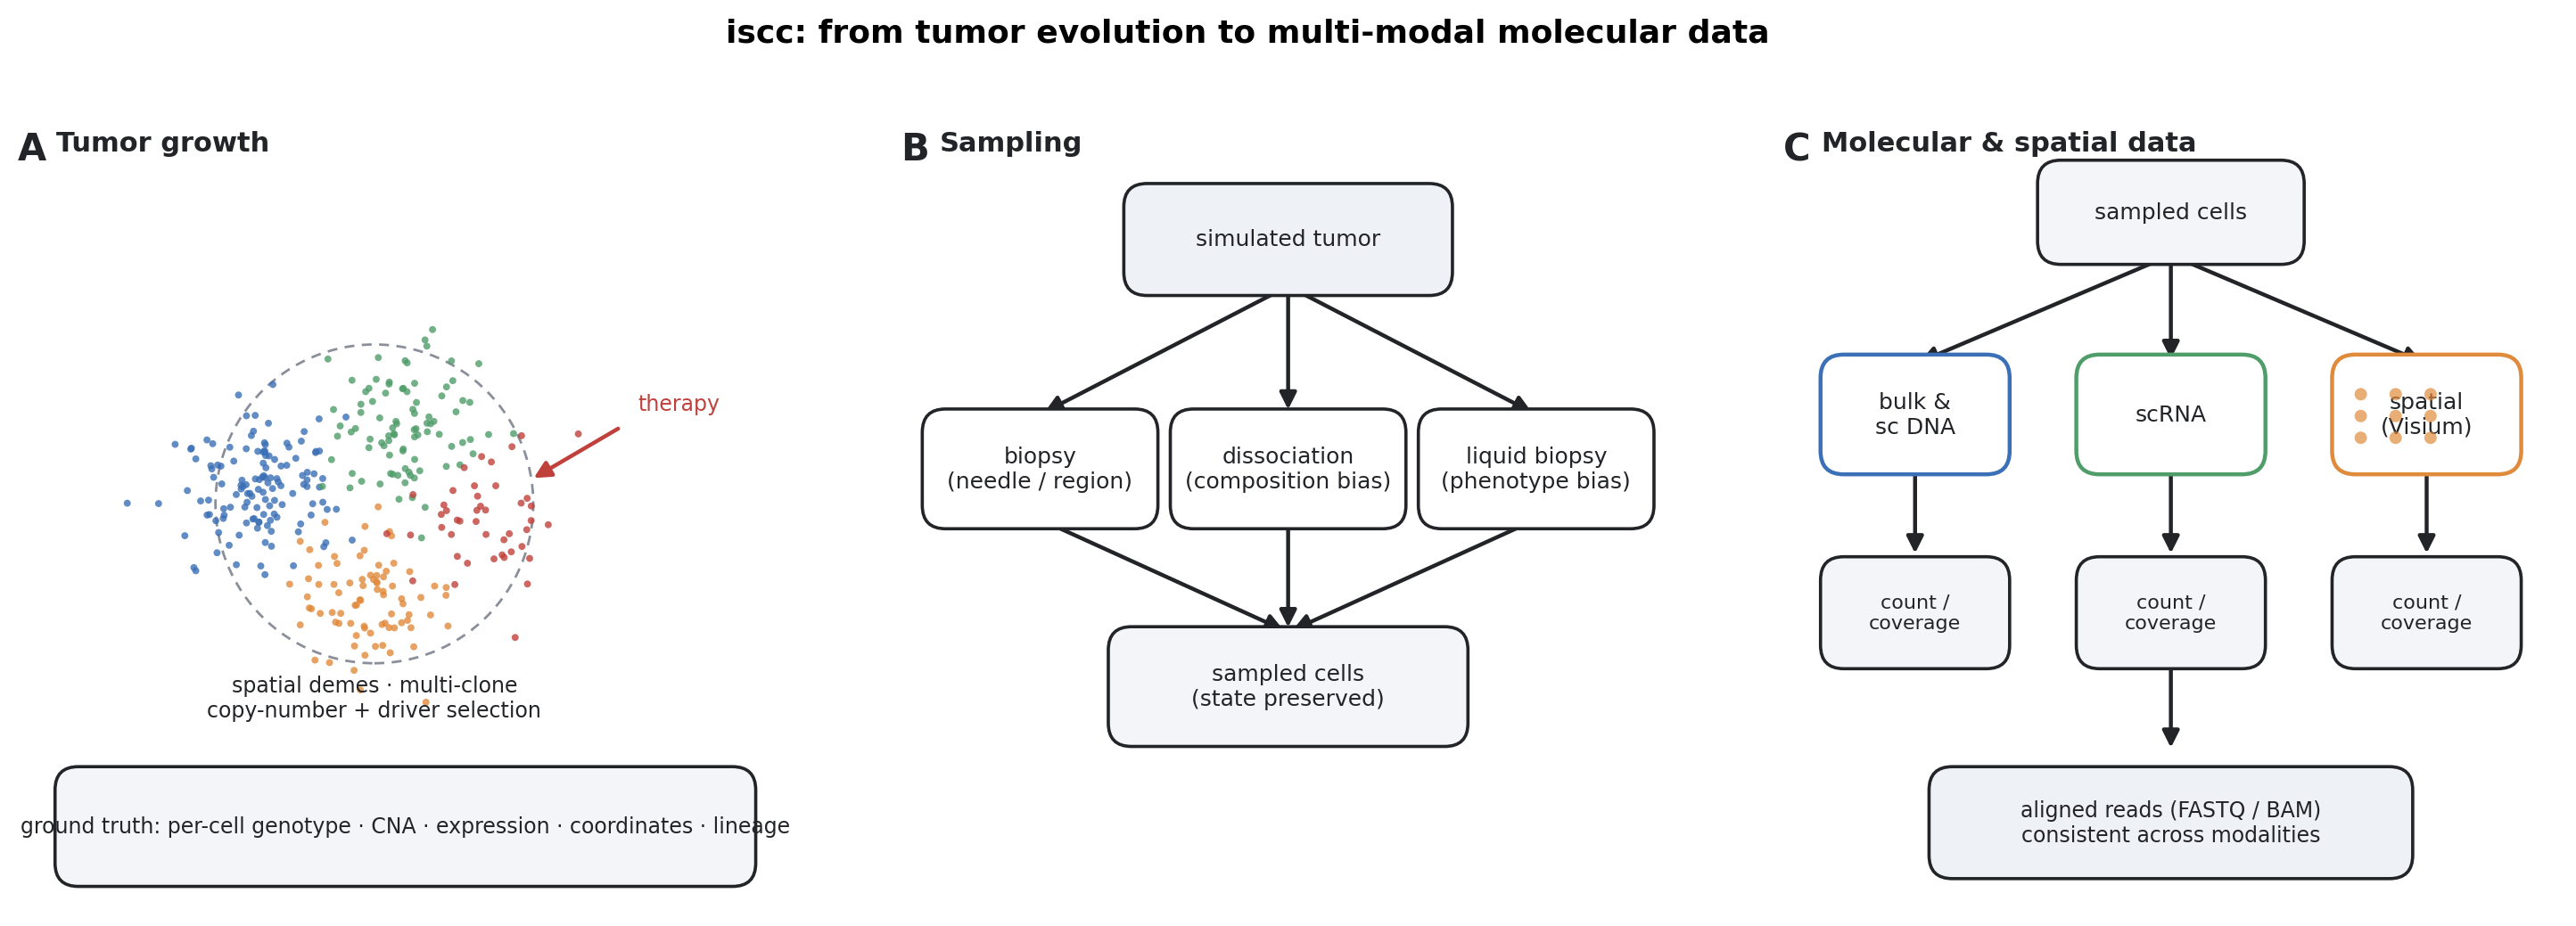
\includegraphics[width=\textwidth]{overview.png}
  \caption{\textbf{Overview of \texttt{iscc}.} (A) The tumor module grows a spatially
  structured tumor of multiple cell types under a copy-number and driver-mutation selection
  model, producing ground-truth per-cell genotypes, copy numbers, expression and spatial
  coordinates. (B) The sample module performs biopsy and dissociation. (C) The data module
  generates bulk and single-cell DNA and RNA sequencing and spot-based spatial
  transcriptomics. The treatment module can be applied during growth.}
  \label{fig:overview}
\end{figure}

\subsection*{\texttt{iscc} simulates tumors with realistic growth dynamics}
\label{sec:tumor}
The model simulates cells with multiple phenotypes that influence the evolutionary dynamics of
the tumor, including normal epithelial and stromal cells and, optionally, immune cells. The
spatial model can be initialized to a specific normal-tissue structure, such as ducts formed of
epithelial cells, enabling simulation of pre-invasive lesions and their progression.

Cancer-cell fitness follows a copy-number-aware selection model in the spirit of
CINner~\cite{dinh_cinner_2025}: oncogene and tumor-suppressor copies and mutations modulate the
division rate, while focal amplifications, deletions and single-nucleotide variants accumulate
along the lineage. Selection is expressed relative to the wild-type genome, so that the
configured baseline rates are recovered in the absence of driver events and only deviations
(driver mutations and copy-number changes) shift fitness.

A central prediction of spatial models of tumor evolution is that the manner of cell dispersal
governs the mode of evolution~\cite{noble_spatial_2022}. We recapitulate this in \texttt{iscc}
by sweeping the cell dispersal rate and measuring two mode indices over replicate simulations
(\Cref{fig:validation_evolution}): clonal diversity (the Shannon entropy of clone frequencies)
and spatial clonal assortment (whether neighbouring regions are dominated by the same clone).
As dispersal increases, clonal diversity falls monotonically (Shannon $5.8 \to 2.7$) while
spatial assortment rises ($0.21 \to 0.61$): low dispersal produces a finely intermixed, highly
diverse mosaic of local lineages, whereas high dispersal yields fewer clones expanding into
spatially coherent patches (clonal sweeps), consistent with~\cite{noble_spatial_2022}.

We further validated the single-nucleotide variants accumulated along the lineages against
neutral population-genetics theory. Under neutral tumor growth, the bulk variant-allele-frequency
(VAF) distribution is dominated by rare variants and its cumulative form follows the $1/f$ power
law $M(f) = (\mu/\beta)(1/f - 1/f_{\max})$~\cite{williams_identification_2016}. Growing neutral
tumors in \texttt{iscc} (all driver, dispersal and resistance effects set to one, so every
mutation is a passenger) and reading out the population VAF that a bulk assay would observe, we
find a rare-variant-dominated spectrum whose cumulative form is well approximated by the neutral
$1/f$ law over the subclonal range (mean $R^2 = 0.88 \pm 0.04$ over replicates;
\Cref{fig:validation_snv}). Because \texttt{iscc} is spatially explicit, the spectrum also shows
the depletion of intermediate-frequency variants reported for spatially constrained tumors, in
which local growth prevents subclones from sweeping the whole lesion~\cite{sun_between-region_2017,
chkhaidze_spatially_2019}.

We also validated the copy-number alterations against the selective pressures that shape cancer
genomes, which recurrently amplify oncogenes and delete tumor suppressors rather than drifting
neutrally~\cite{beroukhim_landscape_2010,davoli_cumulative_2013}. Under the CINner-style
selection model, a segment's population copy number should rise with its net oncogenic content
(oncogene minus tumor-suppressor positions). Pooling per-segment copy number against net
oncogenic content over replicate tumors, we find a positive relationship under selection that is
absent under neutral drift (\Cref{fig:validation_cna}). The effect size is modest because
copy-number events act per segment while drivers are distributed within segments --- amplifying a
segment helps its oncogenes but also its tumor suppressors --- so the neutral-versus-selection
contrast, rather than the absolute slope, is the signature. Further biological validation --- of
cell-type spatial composition and expression states --- is ongoing and follows the same
replicate methodology.

\begin{figure}[t]
  \centering
  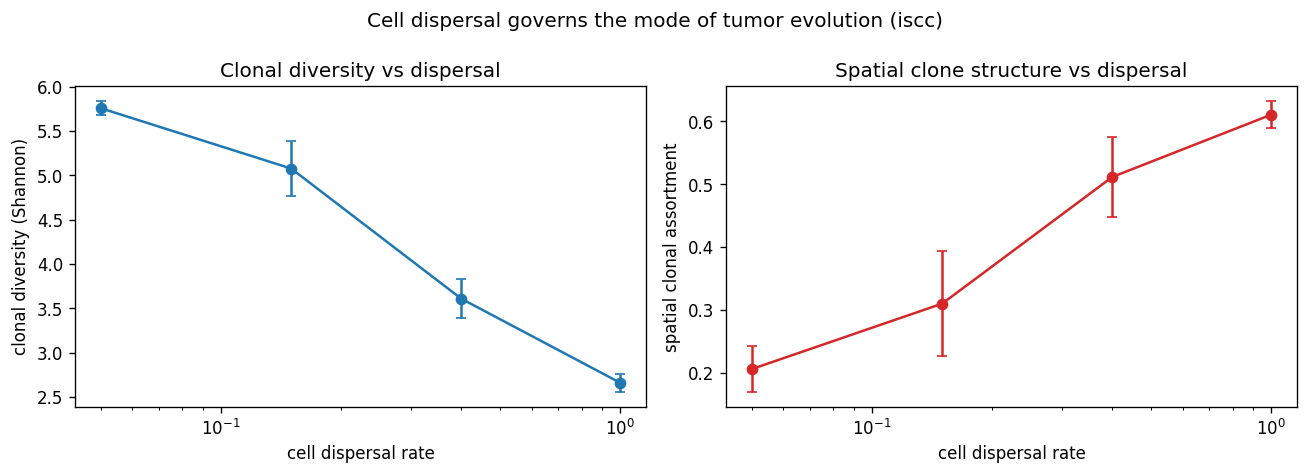
\includegraphics[width=\textwidth]{validation_evolution.png}
  \caption{\textbf{Cell dispersal governs the mode of tumor evolution.} Sweeping the cell
  dispersal rate in \texttt{iscc} (mean $\pm$ s.d. over replicate simulations): clonal
  diversity (Shannon entropy of clone frequencies) decreases with dispersal, while spatial
  clonal assortment (fraction of neighbouring regions sharing the dominant clone) increases.
  Low dispersal yields a diverse, finely intermixed mosaic; high dispersal yields fewer,
  spatially coherent clonal expansions --- recapitulating~\cite{noble_spatial_2022}.}
  \label{fig:validation_evolution}
\end{figure}

\begin{figure}[t]
  \centering
  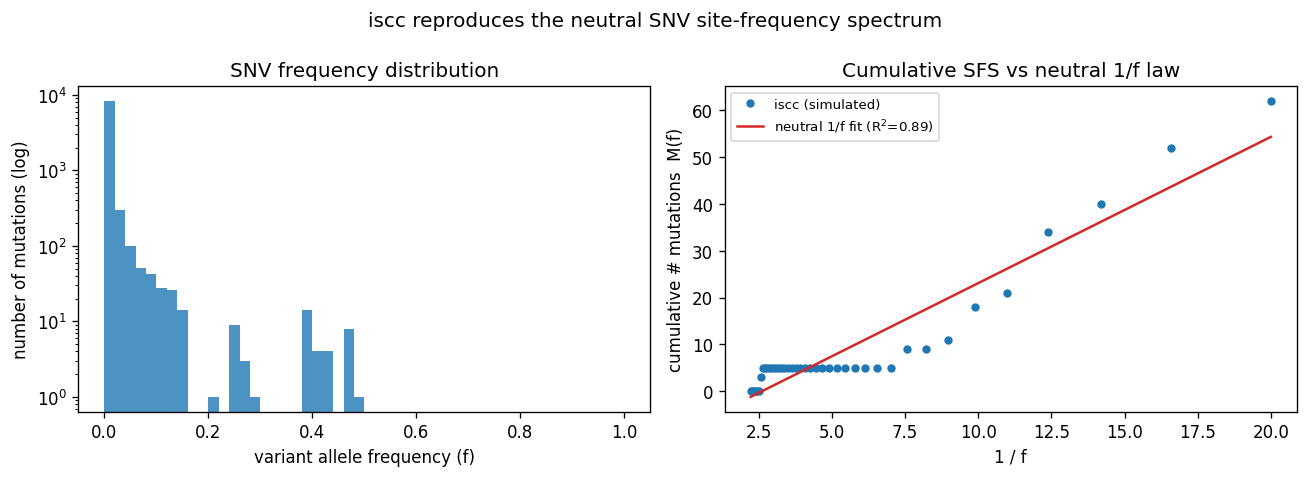
\includegraphics[width=\textwidth]{validation_snv.png}
  \caption{\textbf{Neutral SNV site-frequency spectrum.} Single-nucleotide variants accumulated
  by \texttt{iscc} under neutral growth. Left: the bulk variant-allele-frequency distribution is
  dominated by rare variants. Right: the cumulative number of mutations $M(f)$ is linear in $1/f$,
  matching the neutral $1/f$ power law~\cite{williams_identification_2016} ($R^2 = 0.88 \pm 0.04$
  over replicates), with deviations consistent with spatially constrained
  growth~\cite{sun_between-region_2017,chkhaidze_spatially_2019}.}
  \label{fig:validation_snv}
\end{figure}

\begin{figure}[t]
  \centering
  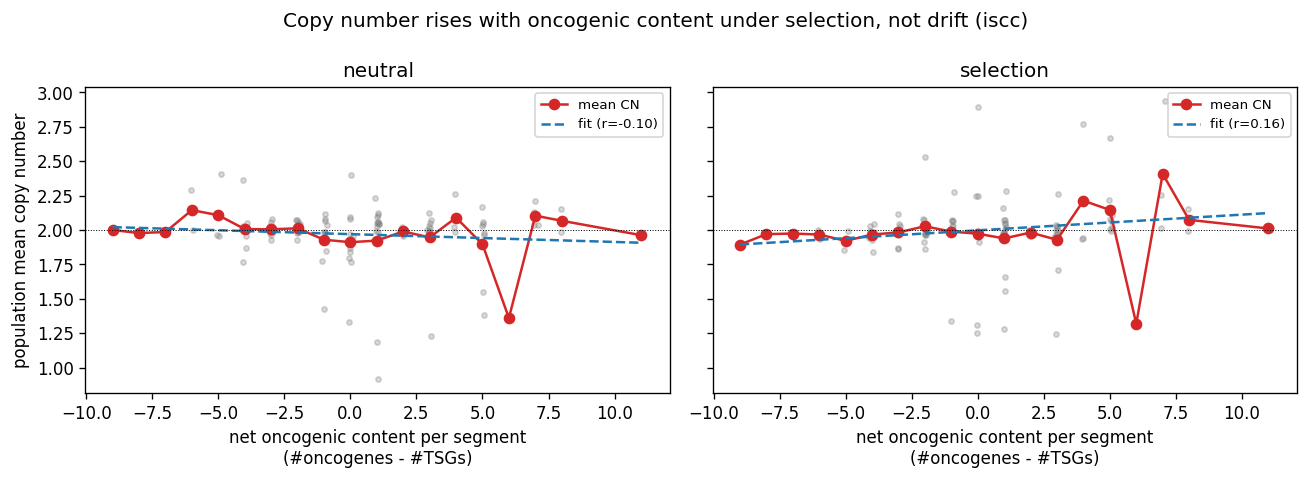
\includegraphics[width=\textwidth]{validation_cna.png}
  \caption{\textbf{Copy-number alterations follow oncogenic selection.} Per-segment population
  copy number versus net oncogenic content (oncogene minus tumor-suppressor positions), pooled
  over replicate tumors. Under neutral drift (left) there is no relationship; under selection
  (right) copy number rises with oncogenic content, recapitulating the recurrent amplification of
  oncogenes and deletion of tumor suppressors seen in cancer
  genomes~\cite{beroukhim_landscape_2010,davoli_cumulative_2013}.}
  \label{fig:validation_cna}
\end{figure}

\subsection*{\texttt{iscc} generates multi-modal molecular and spatial data}
\label{sec:data}
The data module turns the cell populations captured by a biopsy or dissociation into observed
molecular data. For bulk and single-cell DNA sequencing, it generates per-gene coverage and
variant-allele counts with configurable false-positive and false-negative rates, from which
variant-allele frequencies and copy-number profiles can be derived; the compact genome
representation also stores explicit per-position alleles, providing the foundation for future
read-level (FASTQ/BAM) output. For single-cell RNA sequencing, the module generates transcript
counts with cell-to-cell variation in library size and negative-binomial overdispersion. For
spatial data, the module mimics the 10x Visium platform, placing spots over the biopsied tissue
slice and aggregating the transcripts of the cells within each spot.

To verify that the simulated single-cell data are realistic, we compared \texttt{iscc}'s
scRNA-seq output to a real 10x dataset (PBMC3k) using standard count-realism statistics
(\Cref{fig:validation_scrna}). The simulated data reproduce the variation in library size
across cells (coefficient of variation $0.40$ vs $0.46$ in real data), the mean--variance
overdispersion relationship, and the increase of dropout with decreasing mean expression. As
expected, the abstract gene model and smaller synthetic genome yield somewhat denser data than
a genome-wide assay; capturing the full sparsity of genome-wide measurements is a direction for
future work.

\begin{figure}[t]
  \centering
  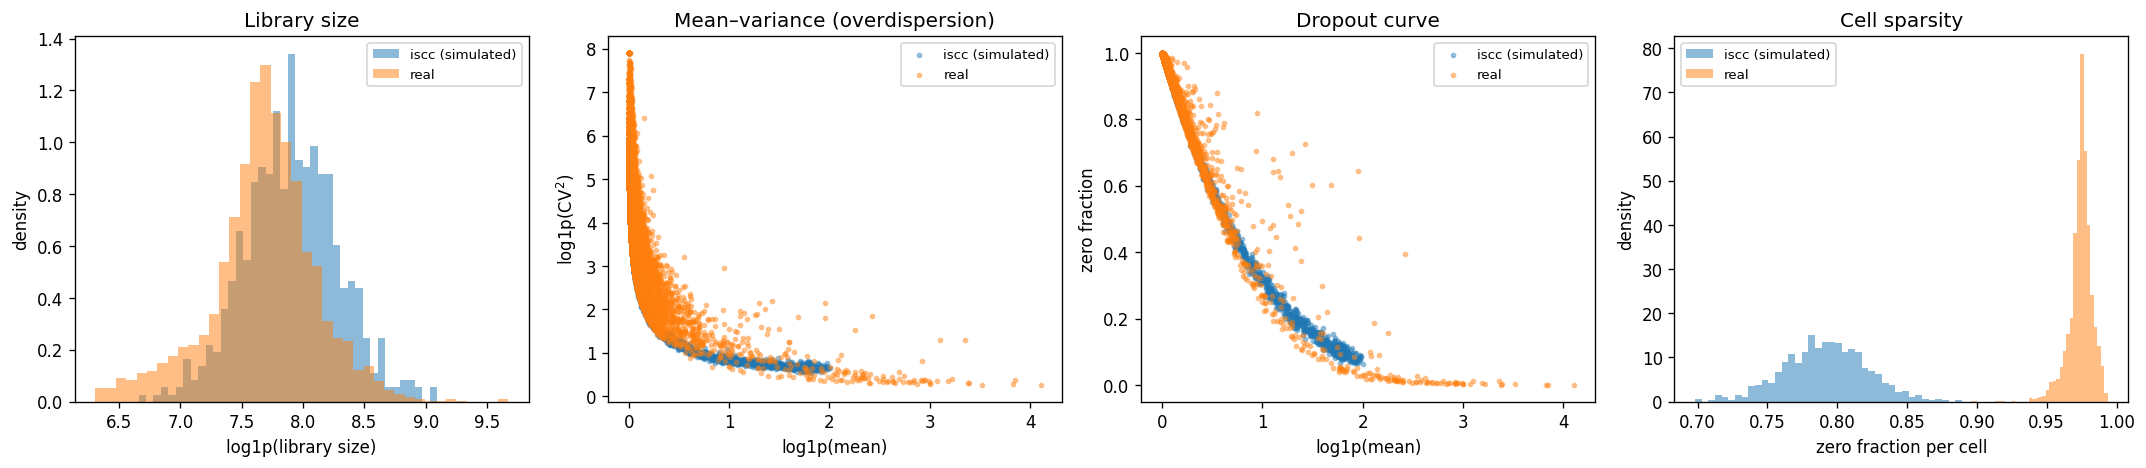
\includegraphics[width=\textwidth]{validation_scrna.png}
  \caption{\textbf{Validation of simulated scRNA-seq against real data.} Count-realism
  statistics for \texttt{iscc} (simulated) overlaid on a real 10x dataset (PBMC3k): per-cell
  library size, the mean--variance (overdispersion) relationship, the dropout curve
  (zero fraction vs mean expression), and per-cell sparsity. \texttt{iscc} reproduces variable
  library size and overdispersion, in contrast to the fixed-depth, underdispersed counts of a
  plain multinomial model.}
  \label{fig:validation_scrna}
\end{figure}

\subsection*{\texttt{iscc} implements conventional and adaptive therapy strategies}
\label{sec:treatment}
A central goal in computational oncology is to use detailed molecular profiles of tumors to
propose treatments tailored to each tumor. \texttt{iscc} includes a treatment module with
chemotherapy, targeted therapy and immunotherapy, applied as the tumor evolves on the default
genotype engine and optionally scheduled as an adaptive regimen that modulates dosing in
response to tumor burden~\cite{west_survey_2023}. Death-rate therapies (chemotherapy and
targeted therapy) impose a kill hazard on sensitive cells, attenuated by each cell's evolved
treatment resistance; immunotherapy instead strips immune resistance so that the local immune
microenvironment kills more, coupling its efficacy to immune cell density and proximity.
Targeted therapy and immunotherapy can be restricted to cells expressing specific genes,
coupling response to the simulated phenotype.

We illustrate this on a sensitive tumor grown to an established burden and then continued under
three regimens (\Cref{fig:treatment}). Without treatment the tumor keeps growing; continuous
chemotherapy regresses it to elimination; and an adaptive regimen that doses only above a burden
threshold holds the tumor in check while delivering substantially less drug (here $\sim$36\%
fewer dosed steps). Because \texttt{iscc} records the full pre- and post-treatment clone history,
it can be used to study therapy-induced resistance and to compare continuous and adaptive
strategies on a shared evolutionary ground truth.

\begin{figure}[t]
  \centering
  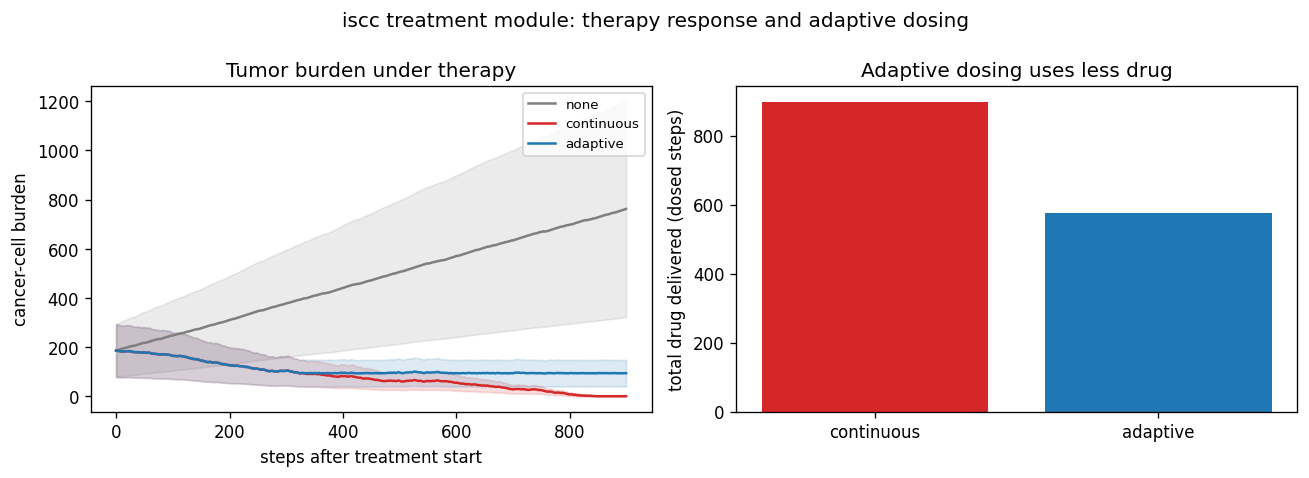
\includegraphics[width=\textwidth]{validation_treatment.png}
  \caption{\textbf{Treatment in \texttt{iscc}.} A sensitive tumor is grown to an established
  burden, then continued under three regimens (mean $\pm$ s.d. over replicate simulations).
  Left: cancer-cell burden over time --- untreated tumors grow, continuous chemotherapy
  regresses the tumor, and adaptive chemotherapy controls it near the dosing threshold. Right:
  total drug delivered; the adaptive regimen achieves control with markedly less drug than
  continuous dosing~\cite{west_survey_2023}.}
  \label{fig:treatment}
\end{figure}


\section*{Methods}
\label{sec:methods}
In the following we outline the modules that constitute the package: tumor, treatment, sample
and data.

\subsection*{The \texttt{tumor} module}
This module contains the building blocks of a tumor as classes: \texttt{Genome},
\texttt{Cell}, \texttt{Deme} and \texttt{Selection}. A tumor can be instantiated as a glandular
(spatially structured) model. Demes are arranged on a 2D grid; each holds cells up to a
carrying capacity, and cells divide, die and disperse to neighboring demes at rates determined
by their genotype and local environment. The genome of each cell is represented compactly, with
copy number tracked per segment and single-nucleotide variants stored as per-position bitsets
under an infinite-sites assumption. We follow the copy-number and driver-mutation selection
model developed in CINner~\cite{dinh_cinner_2025}: oncogene and tumor-suppressor wild-type and
mutated copies, normalized by ploidy, multiplicatively modulate the division rate, and analogous
terms govern dispersal and resistance phenotypes. To scale, the simulation is run at the level
of genotypes: identical cells of a clone in a deme are represented by a count over a shared
genotype, and the per-cell matrices required for data generation are materialized on demand.

\subsection*{The \texttt{treatment} module}
This module includes chemotherapy, targeted therapy and immunotherapy. Each treatment is applied
during \texttt{tumor.grow()} according to a dosing schedule. At the genotype level the per-cell
stochastic effect becomes a dose-scaled modifier of a clone's effective rates, refreshed each
treated step so it never corrupts the shared genotype: death-rate therapies add a kill hazard to
sensitive clones (scaled by dose, drug effectiveness and $1-\text{treatment resistance}$), while
immunotherapy lowers a clone's immune resistance so the local immune microenvironment kills more.
Immune killing itself is modelled as additive contact pressure that rises with local immune-cell
density and is attenuated by immune resistance; the immune compartment is currently static, with
recruitment and migration dynamics left for future work. Treatments can be configured as adaptive
regimens that adjust dosing in response to tumor burden~\cite{west_survey_2023}.

\subsection*{The \texttt{sample} module}
This module corresponds to processing a tumor to prepare it for a data assay, via
\texttt{Biopsy} and \texttt{Dissociation} steps that select a subset of cells from the
simulated tumor while preserving their ground-truth state.

\subsection*{The \texttt{data} module}
The data module generates data from the cells obtained through a biopsy or dissociation of the
simulated tumor. This includes bulk and single-cell DNA and RNA sequencing, as well as
spot-based spatial transcriptomics following the 10x Visium technology. Bulk and single-cell
DNA assays generate coverage and variant-allele counts with configurable error rates.
Single-cell RNA-seq counts are generated with a variable library size (lognormal) and
negative-binomial (gamma--Poisson) overdispersion, so that simulated counts exhibit the
cell-to-cell depth variation and overdispersion of real data. Spatial transcriptomics
aggregates the transcripts of cells falling within each spot of a regular grid placed over the
tissue slice.

\subsection*{Validation}
\label{sec:validation}
We validate simulated single-cell RNA-seq against a real 10x reference dataset using
count-realism summary statistics --- per-cell library size, the mean--variance relationship,
and the dropout (zero fraction vs mean) curve --- computed by the package's \texttt{validation}
module (\Cref{fig:validation_scrna}). The validation script is distributed with the software and
can be pointed at any reference dataset.


\section*{Code availability}
\texttt{iscc} is freely available as a Python package at \url{https://github.com/pedrofale/iscc}.
Detailed documentation and examples are available at \url{https://pedrofale.github.io/iscc}.

\section*{Competing interests}
The authors declare that they have no competing interests.

\section*{Acknowledgements}
The authors would like to thank colleagues at the Department of Biosystems Science and
Engineering, ETH Zurich, for helpful discussions.

\bibliographystyle{unsrt}
\bibliography{references}

\end{document}
